\documentclass{experimentreport}

\input{listing_style.tex}
\usepackage{amsmath}
\usepackage{booktabs}
\usepackage{caption}
\usepackage{float}
\usepackage{graphicx}
\usepackage{tikz}
\usetikzlibrary{arrows.meta,positioning,shapes.geometric}

%========================
% 基本信息
%========================

\setcoursename{基础软件开发技术实践}
\setreportname{智能软件工程实验报告}

\setexperimenttitle{实验七：本地 Web 智能代码审查工作台}

\setstudentname{\hintholder{王皓}}
\setdepartment{\hintholder{计算学部}}
\setstudentid{\hintholder{2023111825}}

\setcourseteacher{刘佳琨}
\setinstructor{刘佳琨}

\setlablocation{\hintholder{格物213}}
\setlabtime{    \hintholder{2026年7月9日}}

\begin{document}

%========================
% 自动生成封面
%========================

\makereporthead

%========================
% 实验目的
%========================

\experimentpurpose{

前六次实验分别完成了代码审查数据构建、传统机器学习合并预测、大语言模型审查、AI 生成代码泛化分析以及上下文与提示策略优化，但这些能力主要以离线脚本和实验矩阵存在，尚未形成可嵌入真实开发过程的软件工具。本实验面向这一“算法验证到工程部署”的缺口，将实验二、四、五、六的模型能力集成为一个浏览器可访问的本地 Web 代码审查工作台，使开发者能够在提交代码或创建 Pull Request（PR）之前，对当前 Git 工作树的修改执行统一、可定位且可追溯的审查。

实验指导书要求实现 VSCode 插件，并完成当前文件获取、代码修改提取、模型调用、Merge Prediction、审查意见展示、历史记录和结果可视化。经实验方案允许，本实验将交互载体由 VSCode Extension 调整为 FastAPI 托管的本地 Web 应用，但保持“前端交互层--HTTP 服务层--模型层”的核心体系不变。该调整降低了插件运行时与打包链路带来的部署成本，同时保留了指导书要求的功能语义、模型集成方式和工程验证目标。

本实验的具体目标如下：

\begin{enumerate}
	\item 建立受启动参数锁定的本地 Git 工作区，在不修改源文件的前提下，可靠发现相对 \texttt{HEAD} 的已暂存、未暂存和未跟踪文本修改，并以统一 diff 展示当前文件与全部修改；
	\item 设计版本化 HTTP API，将工作区发现、安全预检、上下文构建、模型推理、历史持久化和导出组织为边界清晰的软件服务；
	\item 集成 DeepSeek 大语言模型与实验二的 SVM、Random Forest、XGBoost、LightGBM 四个 \texttt{pre-review} 模型，同时明确主审查结论与传统模型实验外迁移参考之间的证据层级；
	\item 通过确定性快照、敏感信息阻断、上下文预算、结构化输出校验、意见定位和保守汇总，提高外部模型调用的一致性、安全性与可解释性；
	\item 实现面向开发者工作流的三栏审查界面和历史界面，并使用离线 API 测试与浏览器端到端测试验证主要功能、异常状态及响应式布局。
\end{enumerate}

本实验将输出限定为“合并就绪度”，即判断当前本地修改是否具备进入提交或 PR 流程的条件。由于本地工作树不包含 PR 标题、讨论过程、维护者决策等平台信息，该结论不等价于 GitHub 最终 Merge 状态预测。这一边界保证了系统表述与可获得证据相一致。

}

%========================
% 实验内容
%========================

\experimentcontent{

\subsection{需求分析与任务边界}

本实验首先将指导书中的插件功能转换为可验收的软件需求。输入对象为启动时锁定的、具有有效 \texttt{HEAD} 的 Git 工作树；审查范围为用户选中的当前修改文件或整个工作区；核心输出包括 MERGE/REJECT 合并就绪度、low/medium/high 风险等级、最多五条带文件与修改后行号的审查意见、覆盖信息、传统模型参考以及调用元数据。系统不提供源码编辑、自动补丁应用或自动提交功能，从而将职责严格限制在“读取--分析--反馈”阶段。

表~\ref{tab:req-map} 给出了指导书要求与本实验实现之间的对应关系。交互载体虽然发生变化，但当前文件、代码修改、模型通信、结果可视化和历史记录等核心能力均被保留；其中浏览器修改列表中的选中项承担“当前编辑文件”的语义，FastAPI API 则承担插件与 Python 后端之间的 HTTP 通信边界。

\begin{table}[H]
	\centering
	\caption{实验指导书功能要求与本地 Web 工作台实现映射}
	\label{tab:req-map}
	\small
	\begin{tabularx}{\textwidth}{p{3.2cm}X X}
		\toprule
		指导书要求 & 本实验实现 & 验收证据 \\
		\midrule
		获取当前编辑文件 & 修改文件列表中的当前选中项 & 单文件 diff 与单文件审查 \\
		获取代码修改内容 & 读取 \texttt{HEAD} 到工作树的统一 diff & staged、unstaged、未跟踪文件测试 \\
		调用代码审查模型 & 浏览器经 \texttt{/api/v1} 调用 LLM 与传统模型 & 预检、审查和健康检查接口 \\
		展示 Merge Prediction & 展示有语义边界的 MERGE/REJECT 合并就绪度 & 主结论、风险和理由区域 \\
		生成审查意见 & 返回经路径和修改后行号校验的结构化 finding & 点击意见定位 diff \\
		历史代码审查记录 & JSONL 存储、筛选、删除和 JSON/Markdown 导出 & History 页面与导出接口 \\
		结果可视化 & 三栏布局、状态图标、风险分级、diff 高亮和调用信息 & 桌面及窄屏浏览器测试 \\
		\bottomrule
	\end{tabularx}
\end{table}

需求分析进一步识别出三类关键风险。第一，本地 staged 与 unstaged 修改可能在同一文件中重叠，若分别拼接将导致重复审查；因此系统必须计算 \texttt{HEAD -> worktree} 的最终净差异。第二，代码需要发送至外部模型，路径逃逸、密钥文件和正文凭据均可能造成信息泄漏；因此外发前必须执行不可绕过的安全预检。第三，模型调用期间文件可能继续变化；因此审查结论必须与确定性快照绑定，并在输入变化后标记为过期，而不能继续作为当前代码的结论。

\subsection{总体架构与技术路线}

系统采用单进程、分层式本地 Web 架构，如图~\ref{fig:architecture} 所示。表现层使用原生 HTML、CSS 和 JavaScript ES modules，负责修改文件导航、只读 diff、审查结果与历史交互；接口层由 FastAPI 提供统一的 \texttt{/api/v1} 契约并托管静态资源；领域服务层负责 Git 快照、安全预检、上下文构建、审查编排和历史管理；外部资源层连接 DeepSeek OpenAI 兼容接口、实验二模型资产、本地 Git 命令和 JSONL 文件。该架构延续了指导书提出的前后端分离思想，同时无需单独部署 Node.js 服务，降低了课程实验的环境复杂度。

\begin{figure}[H]
	\centering
	\resizebox{0.96\textwidth}{!}{%
	\begin{tikzpicture}[
		node distance=0.75cm and 0.55cm,
		box/.style={draw, rounded corners=2pt, align=center, minimum height=1.05cm, text width=3.05cm, fill=gray!6},
		service/.style={box, fill=cyan!8},
		resource/.style={box, fill=orange!9},
		arrow/.style={-{Latex[length=2.2mm]}, thick}
	]
		\node[box] (ui) {浏览器工作台\\Review / History};
		\node[service, right=of ui] (api) {FastAPI 接口层\\\texttt{/api/v1}};
		\node[service, right=of api] (engine) {审查编排层\\ReviewEngine};
		\node[service, below=of api] (workspace) {工作区与上下文\\Snapshot / Preflight};
		\node[resource, below=of ui] (git) {本地 Git 工作树\\\texttt{HEAD -> worktree}};
		\node[resource, below=of engine] (models) {DeepSeek + 实验二\\四个 pre-review 模型};
		\node[resource, right=of engine] (history) {JSONL 历史\\缓存与导出};
		\draw[arrow,<->] (ui) -- node[above, font=\small]{HTTP/JSON} (api);
		\draw[arrow] (api) -- (engine);
		\draw[arrow] (api) -- (workspace);
		\draw[arrow] (workspace) -- (git);
		\draw[arrow] (engine) -- (models);
		\draw[arrow,<->] (engine) -- (history);
		\draw[arrow] (workspace) -- (engine);
	\end{tikzpicture}
	}
	\caption{本地 Web 智能代码审查工作台总体架构。浏览器只通过版本化 HTTP API 访问锁定工作区；领域服务负责在模型调用前建立快照和安全边界。}
	\label{fig:architecture}
\end{figure}

技术选型遵循可复现性与最小部署原则：运行环境为 Python 3.12，并由 \texttt{uv} 统一管理依赖；FastAPI 与 Pydantic 分别承担 HTTP 路由和结构化数据校验；Uvicorn 默认仅监听 \texttt{127.0.0.1}；前端不依赖 CDN 或构建器；历史采用 UTF-8 JSONL 存储，避免为单用户本地工具引入数据库。测试以 FastAPI \texttt{TestClient} 为主接缝，并使用 Python Playwright 验证真实浏览器交互，从而覆盖从 Git 输入到界面反馈的完整路径。

\subsection{详细设计与实施}

\subsubsection{受约束的工作区与确定性快照}

服务启动时将 \texttt{--repo} 解析为规范绝对路径，并验证其为可读、具有有效 \texttt{HEAD} 且参数路径等于顶层目录的 Git 工作树。后续 API 不接受任意仓库路径，所有文件访问都在该根目录内解析并再次验证。工作区发现使用结构化 Git 状态获取新增、修改、删除和重命名信息；对于受跟踪文件，系统直接生成 \texttt{HEAD} 到当前工作树的统一 diff，使 staged 与 unstaged 修改自然合并；未跟踪文本文件则被建模为空文件到当前文件的新增 diff。

为了使一次审查与确定输入绑定，系统对规范化后的文件顺序、diff、作用域和 \texttt{HEAD} 提交计算 SHA-256。其逻辑可表示为
\[
H = \operatorname{SHA256}(v \Vert c_{\mathrm{HEAD}} \Vert s \Vert D_{\mathrm{sorted}}),
\]
其中 $v$ 为快照模式版本，$c_{\mathrm{HEAD}}$ 为当前提交标识，$s$ 为文件或工作区作用域，$D_{\mathrm{sorted}}$ 为按相对路径稳定排序的规范化差异。前端提交预检或审查时携带最后观察到的 $H$；若服务端重算值不一致，则返回 HTTP 409，要求刷新后重新确认。审查结束后再次计算哈希，可识别推理期间发生的修改并将结果标记为 stale。

\subsubsection{安全预检与外发边界}

预检位于任何付费模型调用之前。系统依次执行仓库内路径约束、符号链接拒绝、常见敏感路径匹配、文件大小与二进制检测、UTF-8 文本读取和正文凭据模式扫描。敏感路径覆盖 \texttt{.env*}、证书与私钥、凭据目录、依赖目录和构建产物；正文扫描覆盖 API key、GitHub token、私钥头、AWS access key、Bearer token 和高置信度密码赋值。命中规则的文件被列入排除报告且不提供绕过开关，错误信息仅返回规则名称而不回显疑似密钥正文。

预检响应同时列出拟送审文件、排除项、上下文来源、总字符数、预计批次和未覆盖项。用户点击审查即表示确认发送该报告所界定的范围。该机制将数据外发从隐式副作用转化为可观察、可阻断和可审计的显式步骤。

\subsubsection{确定性上下文与预算分批}

上下文构建遵循“diff $>$ 修改后文件 $>$ 相关测试 $>$ 符号引用 $>$ 项目约定”的固定优先级。每个批次至少包含文件路径、状态、统一 diff、hunk 标识和修改后行号；Python 文件进一步通过抽象语法树识别发生变更的顶层函数或类，并在仓库中检索同名测试及有限数量的词法引用。项目约定优先读取 \texttt{AGENTS.md}、\texttt{CLAUDE.md}、\texttt{CONTRIBUTING.md} 或 \texttt{README.md} 的预算片段。所有候选按确定性规则排序，使相同快照与配置产生相同上下文。

默认单批字符预算为 48,000。完整文件上下文不能放入当前批次时先按文件边界开启新批；单文件仍超预算时再按 hunk 切分，避免在 diff 元信息或代码行中间截断。系统优先覆盖 Python 文件，最多执行四次代码批审查；其余内容进入 \texttt{unreviewed\_items}，并使总体状态降级为 \texttt{INCOMPLETE}。图~\ref{fig:sequence} 展示了从刷新工作区到结果持久化的完整审查时序。

\begin{figure}[H]
	\centering
	\resizebox{0.96\textwidth}{!}{%
	\begin{tikzpicture}[
		node distance=0.55cm,
		flowstep/.style={draw, align=center, minimum height=0.8cm, text width=10.8cm, fill=gray!5},
		decision/.style={draw, diamond, aspect=4.4, align=center, fill=yellow!12},
		arrow/.style={-{Latex[length=2mm]}, thick}
	]
		\node[flowstep] (discover) {读取 Git 状态并构造 \texttt{HEAD -> worktree} 规范化差异};
		\node[flowstep, below=of discover] (hash) {生成 scope 快照与 \texttt{snapshot\_hash}};
		\node[flowstep, below=of hash] (preflight) {执行路径、敏感内容与预算预检，向用户展示实际发送范围};
		\node[decision, below=0.75cm of preflight] (check) {快照一致且存在可审查内容？};
		\node[flowstep, below=0.75cm of check] (context) {构建确定性上下文并规划最多四个代码批次};
		\node[flowstep, below=of context] (review) {LLM 结构化审查；并行生成实验二传统模型参考};
		\node[flowstep, below=of review] (validate) {校验 JSON、路径与行号，去重排序；多批次执行保守汇总};
		\node[flowstep, below=of validate] (persist) {重算快照判定 stale，写入 JSONL 并返回可视化结果};
		\draw[arrow] (discover) -- (hash);
		\draw[arrow] (hash) -- (preflight);
		\draw[arrow] (preflight) -- (check);
		\draw[arrow] (check) -- node[right, font=\small]{是} (context);
		\draw[arrow] (context) -- (review);
		\draw[arrow] (review) -- (validate);
		\draw[arrow] (validate) -- (persist);
		\draw[arrow] (check.east) -- ++(2.2,0) node[right, align=left, font=\small]{否：返回 409、无修改或\\敏感内容阻断错误};
	\end{tikzpicture}
	}
	\caption{一次代码审查操作的端到端控制流程。快照一致性和安全预检位于模型调用之前，结果校验与过期检测位于持久化之前。}
	\label{fig:sequence}
\end{figure}

\subsubsection{联合 LLM 审查与传统模型参考}

LLM 主审查复用实验四、六的 OpenAI 兼容调用方式，默认使用 DeepSeek V4 Flash 模型。\texttt{strict} 配置采用实验六 P5 Self-Reflection 的核心思想：先主动寻找 blocking defect，再由缺陷证据反推总体结论；\texttt{fast} 配置提供单轮快速审查。模型被要求一次返回 decision、risk level、summary、reasoning、blocking defects 和逐 hunk findings 的 JSON 对象，从而避免分别调用“合并预测”和“意见生成”造成结论不一致。

模型返回后，Pydantic 首先校验枚举和字段结构；解析失败时仅允许一次格式修复。每条 finding 的路径必须属于当前批次，行号必须为空或位于该文件的修改后 hunk 行集合中，否则丢弃并记录警告。有效意见按 blocker、warning、info 以及路径和行号稳定排序，规范化去重后最多保留五条。若任一批次含 blocker，则结论强制为 REJECT 且风险为 high；存在批次失败或未覆盖内容时，总体状态为 INCOMPLETE，不得渲染为可靠 MERGE。多批次汇总只接收批结果和覆盖摘要，不再次发送源码，也不得新增 finding。

传统机器学习区域仅对包含 Python 修改的作用域运行实验二 SVM、Random Forest、XGBoost 和 LightGBM 的 \texttt{pre-review} 模型。系统复用已保存的 scaler、模型权重和固定词表，只执行 \texttt{transform} 与推理，不在当前仓库重新拟合。由于本地输入缺少 PR 标题、正文和审查后过程变量，该结果明确标记为实验外迁移参考，不参与 LLM 的合并就绪度结论；非 Python 修改则仅执行 LLM 降级审查。

\subsubsection{接口、历史与人机交互}

接口统一采用 \texttt{/api/v1} 前缀。表~\ref{tab:api} 概括了主要资源及其职责。写操作使用请求中携带的预期快照哈希实施乐观并发控制；等价的并发审查请求按“快照+配置+作用域+模型”键拒绝重复执行；错误响应统一包含 code、message、details 和 request ID，以支持前端状态呈现和日志追踪。

\begin{table}[H]
	\centering
	\caption{本地代码审查工作台的主要 HTTP API}
	\label{tab:api}
	\small
	\begin{tabularx}{\textwidth}{p{1.6cm}p{4.5cm}X}
		\toprule
		方法 & 路径 & 职责 \\
		\midrule
		GET & \texttt{/api/v1/health} & 返回仓库、LLM、传统模型和历史存储状态 \\
		GET & \texttt{/api/v1/workspace} & 返回当前快照、分支和修改文件列表 \\
		GET & \texttt{/api/v1/diff} & 返回指定修改文件的统一 diff 与 hunk 元数据 \\
		POST & \texttt{/api/v1/preflight} & 生成发送范围、安全排除和批次计划 \\
		POST & \texttt{/api/v1/reviews} & 执行结构化审查并持久化有效结果 \\
		GET & \texttt{/api/v1/progress/\{id\}} & 返回正在执行的批次进度 \\
		GET/DELETE & \texttt{/api/v1/history} & 分页筛选、导出或清空历史 \\
		GET & \texttt{/api/v1/exports/\{id\}.\{format\}} & 导出单次 JSON 或 Markdown 结果 \\
		\bottomrule
	\end{tabularx}
\end{table}

历史记录由后端作为唯一写入方，以 UTF-8 JSONL 保存最近 200 条自包含记录。默认仅保存输入哈希、diff 统计、上下文来源、结构化结论、模型用量和耗时，不保存完整源码；用户显式启用后才保存通过安全检查且受 48,000 字符预算限制的 diff。前端 Review 页在桌面端采用“文件--diff--结果”三栏布局，窄屏切换为三个页签；History 页支持筛选、详情、删除、清空与导出。finding 被点击后，界面滚动并高亮对应修改行，使模型意见能够回到具体代码证据。

}

%========================
% 实验结果
%========================

\experimentresult{

\subsection{系统运行与界面结果}

系统已实现从本地修改发现、预检、模型审查到历史导出的闭环。服务从实验七目录运行 \texttt{uv run python -m src.app serve --repo <git-worktree>} 后，默认监听 \texttt{http://127.0.0.1:8765}；未配置 DeepSeek API key 时服务保持 degraded 状态，工作区、diff、历史和传统模型资产检测仍可使用，而付费主审查按钮被禁用并显示原因。

图~\ref{fig:workbench} 展示了实际运行的 Review 主界面。顶部状态栏同时呈现仓库、分支、修改数量和模型状态；左栏用于选择当前修改文件，中栏以固定行号显示统一 diff，右栏按“合并就绪度--风险与摘要--可定位意见--覆盖和上下文--传统模型参考--调用详情”的顺序组织结果。该层级使 LLM 主结论与传统模型参考保持视觉分离，并允许开发者从 finding 直接返回对应修改行。

\begin{figure}[H]
	\centering
	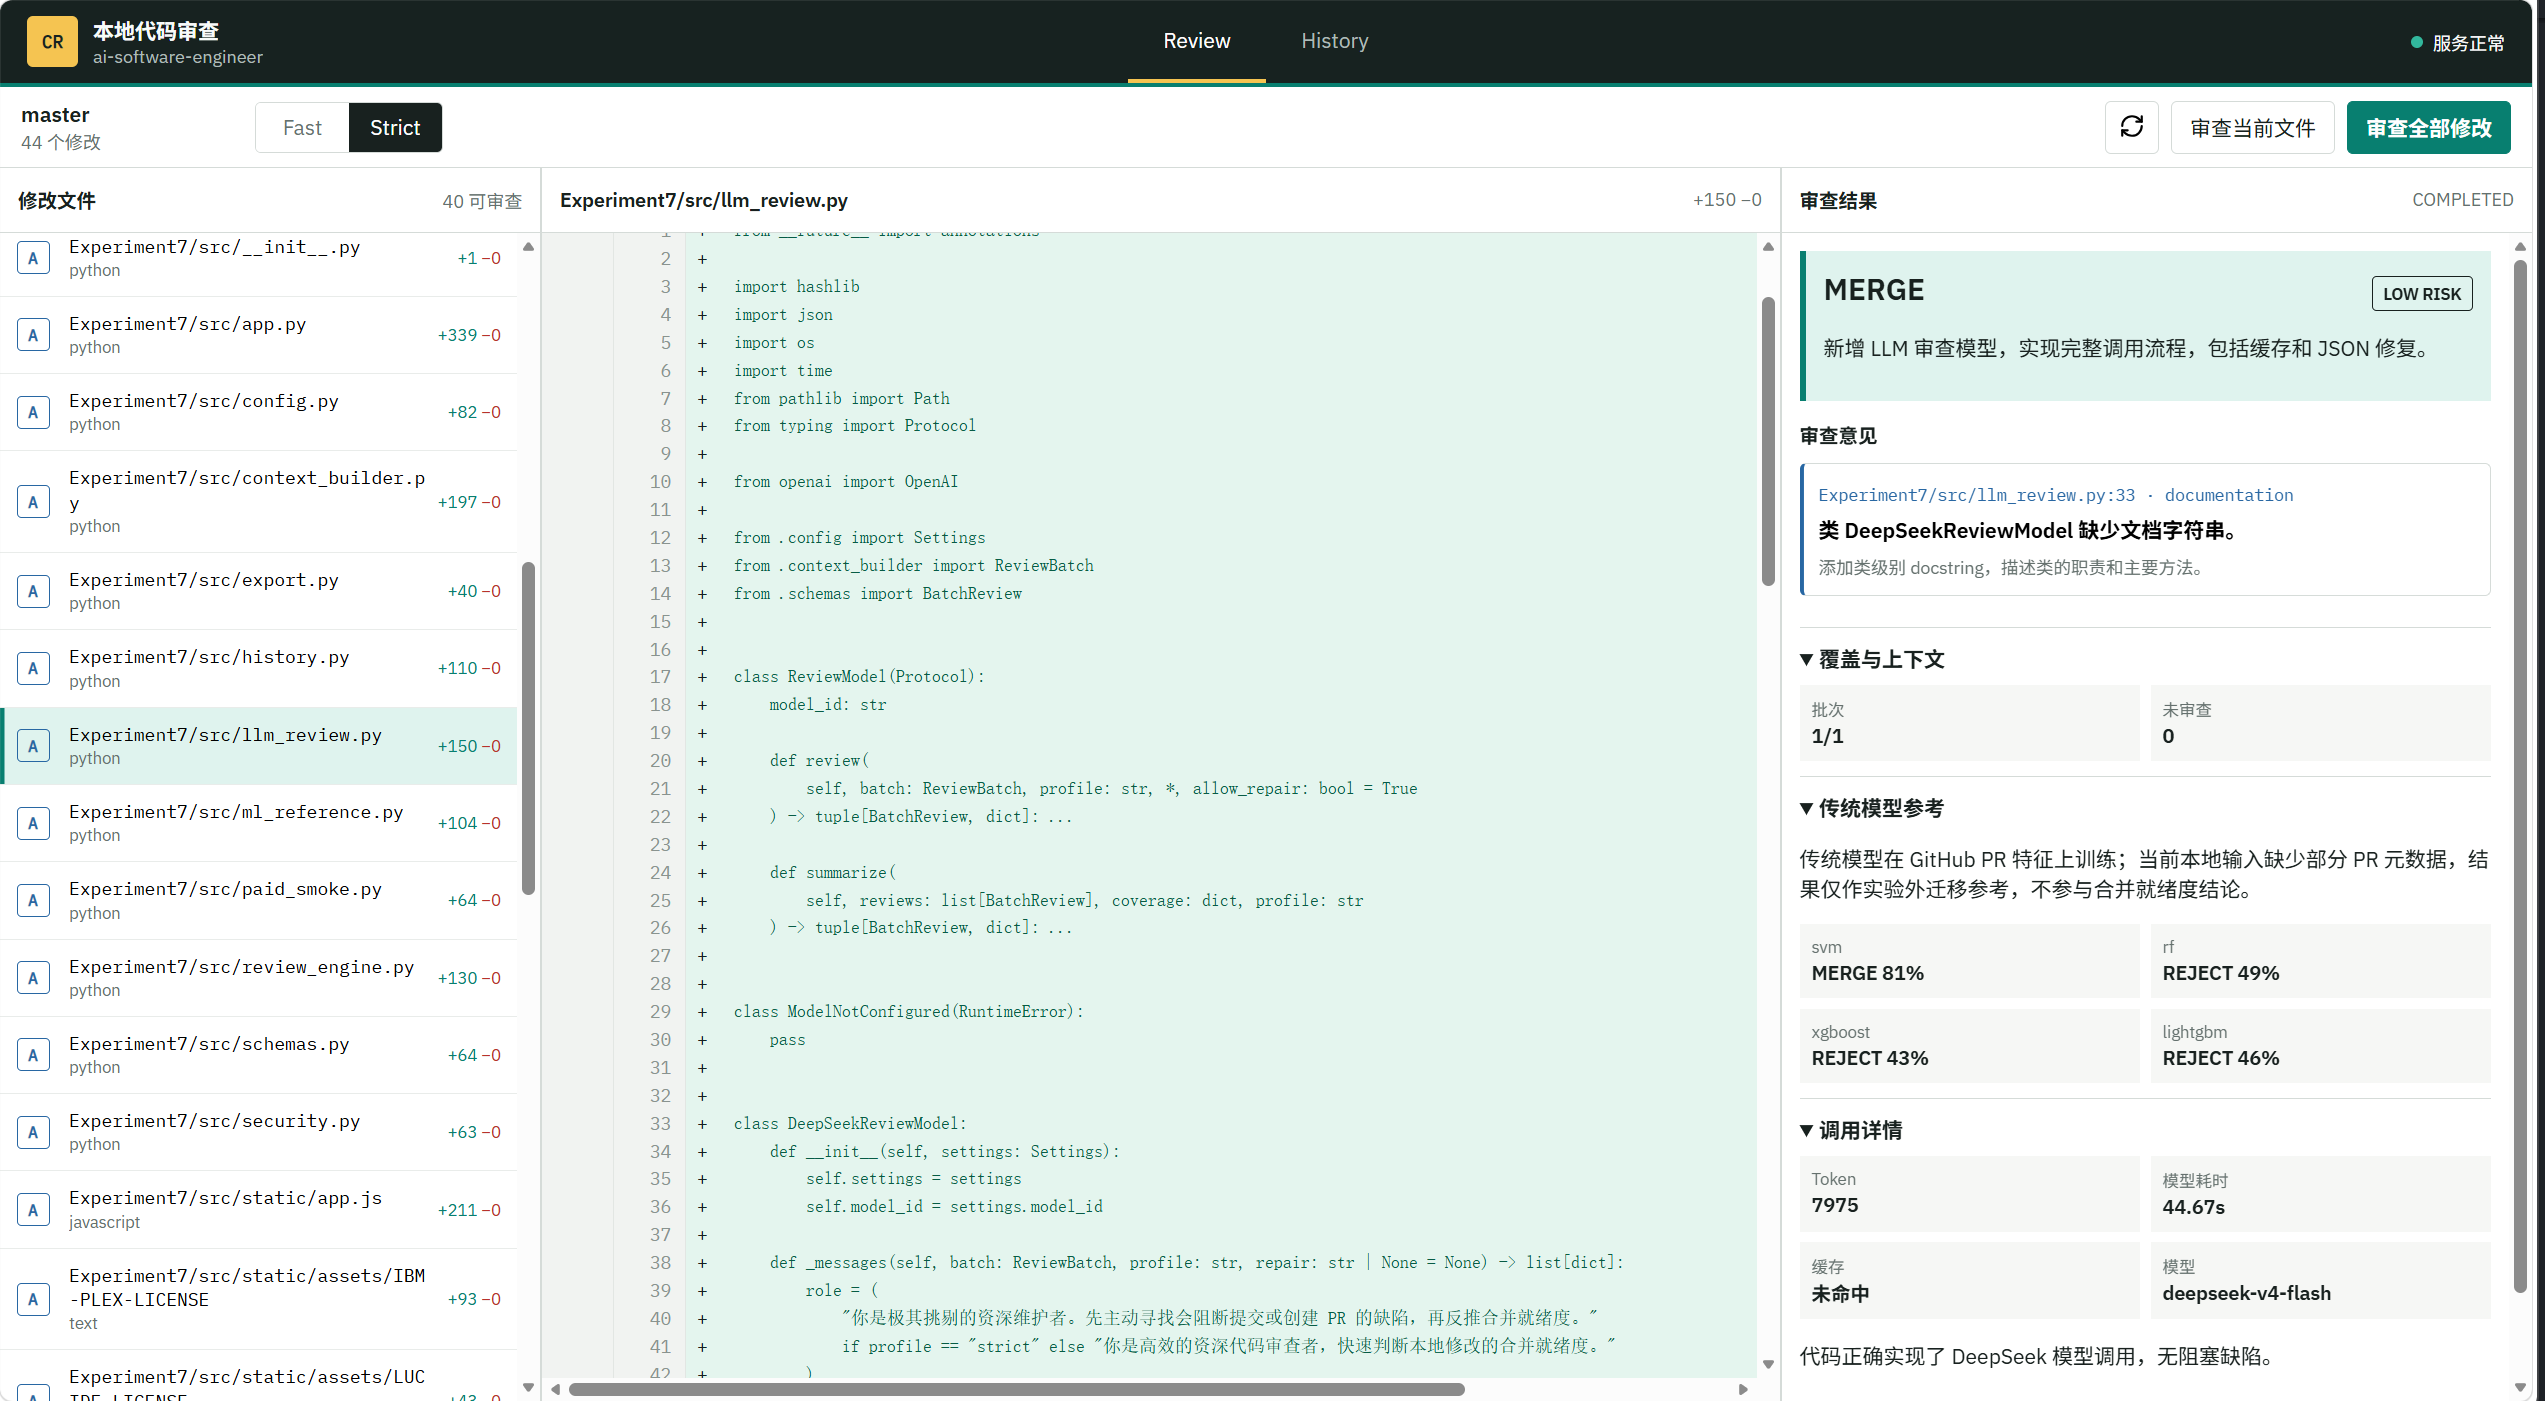
\includegraphics[width=\textwidth]{../results/image/example.png}
	\caption{本地 Web 智能代码审查工作台运行界面。三栏分别呈现修改文件、统一 diff 和结构化审查结果；顶部提供工作区状态、刷新及当前文件/全部修改审查操作。}
	\label{fig:workbench}
\end{figure}

\subsection{功能与鲁棒性验证}

验证采用“真实临时 Git 仓库 + FastAPI TestClient + 确定性 LLM 桩”的离线方案，避免测试产生外部 API 费用，同时保留 Git 命令、HTTP 契约、上下文编排、历史文件和导出逻辑。浏览器层使用 Playwright 启动 Chromium，验证桌面三栏、移动端页签、预检对话框、审查结果渲染和 finding 行定位。表~\ref{tab:verification} 汇总了测试覆盖的主要质量属性与判定条件。

\begin{table}[H]
	\centering
	\caption{实验七功能与异常路径验证矩阵}
	\label{tab:verification}
	\small
	\begin{tabularx}{\textwidth}{p{3.2cm}X X}
		\toprule
		验证维度 & 测试场景 & 通过条件 \\
		\midrule
		工作区正确性 & staged、unstaged、未跟踪、重命名和删除 & 同一文件不重复，状态、增删行和最终净差异正确 \\
		安全性 & 凭据正文、二进制、符号链接和路径逃逸 & 文件被阻断且响应不泄漏敏感正文 \\
		一致性 & 预检后修改文件、审查期间改变工作区 & 前者返回 HTTP 409，后者结果标记 stale \\
		模型约束 & blocker、非法行号、多批次和批次失败 & 强制 REJECT/high，丢弃非法定位，4+1 上限成立 \\
		传统模型 & Python 修改调用四个 pre-review 模型 & 四模型均使用已保存资产完成 transform 与预测 \\
		历史与导出 & 追加超过 200 条、筛选、删除、清空、导出 & 仅保留最近 200 条，JSON/Markdown 内容完整 \\
		浏览器交互 & 桌面与移动视口、finding 点击 & 三栏/页签切换正确，diff 对应行被滚动并高亮 \\
		降级运行 & 未配置 LLM API key & 健康状态为 degraded，非 LLM 功能保持可用 \\
		\bottomrule
	\end{tabularx}
\end{table}

离线测试证明了三个关键工程不变量。其一，审查输入由快照哈希唯一绑定，工作区变化不会被静默忽略。其二，任何含 blocker 的有效批次都不能汇总为 MERGE，任何覆盖不完整的执行都不能显示为可靠 MERGE。其三，安全阻断发生在外部调用之前，且默认历史记录不持久化完整 diff。上述验证共同说明，本系统不仅实现了可见功能，还对输入一致性、结论保守性和代码外发边界进行了可执行约束。

\subsection{指导书目标达成与结果边界}

由表~\ref{tab:req-map} 的需求映射、图~\ref{fig:architecture} 的架构实现、图~\ref{fig:workbench} 的运行界面以及表~\ref{tab:verification} 的验证结果可知，本实验完成了指导书要求的当前文件与修改获取、HTTP 模型通信、Merge Prediction 语义展示、自动审查意见、风险与位置可视化、历史记录和功能测试。与原插件方案相比，本地 Web 方案改变的是界面宿主，而非核心业务流程；统一由 FastAPI 托管前端与接口还减少了独立扩展打包和前端服务部署环节。

结果的适用范围仍受输入和模型证据限制。Python 是经过完整传统模型链路验证的语言；其他文本语言仅支持 LLM 降级审查。相关测试和符号引用采用确定性词法检索，不能替代完整调用图或语义检索。系统面向本机单用户，不提供远程认证与团队协作。最重要的是，本地修改缺少 GitHub PR 的标题、正文、讨论和最终维护决策，因此“合并就绪度”只表示代码进入提交或 PR 流程前的工程准备程度；实验二模型的输出仅用于观察跨场景迁移行为，不构成平台最终合并概率。该限制与系统输入边界一致，也避免了超出实验结果的推断。

}

%========================
% 问题总结
%========================

\experimentproblems{

本实验遇到的第一个问题是 Git 工作区状态具有组合性：同一文件可能同时包含 staged、unstaged 和未跟踪修改，直接分别读取容易产生重复或不一致的审查输入。对此，系统统一计算相对 \texttt{HEAD} 的最终净差异，并通过确定性文件顺序和快照哈希绑定一次审查输入；若预检后工作区发生变化，则返回 HTTP 409，审查期间发生变化则将结果标记为 stale。

第二个问题是将本地代码发送给外部模型可能造成敏感信息泄漏。系统在模型调用前增加不可绕过的安全预检，检查路径、符号链接、二进制文件、敏感路径、文件大小和凭据模式；命中的内容被排除且不回显正文，默认历史记录也不保存完整 diff。该设计将安全约束放在外部调用之前，避免依赖模型自行识别风险。

第三个问题是模型输出可能出现结构不完整或定位不准确。系统使用结构化 JSON 和 Pydantic 校验，并对 finding 的路径及修改后行号进行约束；格式错误最多执行一次修复，非法定位被丢弃。若存在 blocker、批次失败或未覆盖修改，系统分别强制输出 REJECT/high 或 INCOMPLETE，从而避免把不充分证据渲染为可靠的 MERGE。

此外，指导书原方案以 VSCode 插件作为交互载体，而本实验采用本地 Web 工作台实现相同的核心业务流程。该调整减少了插件打包和运行时配置成本，但也意味着本实验没有声称完成 VSCode Extension API 层面的安装验证；当前验证范围是 FastAPI 接口、真实临时 Git 仓库以及浏览器端工作台交互。

}

%========================
% 实验体会
%========================

\experimentexperience{

本实验使我认识到，代码审查模型从离线实验走向可用工具，关键不只是接入模型，而是建立完整的软件工程约束。Git 快照、预检、上下文预算、结构化输出校验、过期检测和历史记录共同决定了审查结果是否可复现、可解释和可追溯；其中任何一个环节缺失，都可能使正确的模型判断失去工程可信度。

前后端分离的本地 Web 架构也体现了较好的迭代性。浏览器负责交互和结果呈现，FastAPI 负责工作区、模型和历史管理，因此模型替换、接口测试与界面调整可以相对独立进行。通过离线桩模型、TestClient 和 Playwright，系统能够在不产生 API 费用的情况下验证主要功能和异常路径，这比只依赖人工截图更能说明实现是否满足需求。

最后，本实验强化了对结果边界的认识。实验二模型的本地推理只能作为跨场景参考，DeepSeek 输出的 MERGE/REJECT 也只表示当前修改的本地合并就绪度，不能替代 GitHub 维护者的最终决策。后续可在保持这一边界的前提下，增加真实 Pull Request 数据接入、更多语言支持、语义级符号检索和团队协作能力。

}

%========================
% 教师评语
%========================

\teachercomment

\end{document}